% Generated by Sphinx.
\def\sphinxdocclass{report}
\documentclass[letterpaper,10pt,english]{sphinxmanual}
\usepackage[utf8]{inputenc}
\DeclareUnicodeCharacter{00A0}{\nobreakspace}
\usepackage{cmap}
\usepackage[T1]{fontenc}
\usepackage{babel}
\usepackage{times}
\usepackage[Bjarne]{fncychap}
\usepackage{longtable}
\usepackage{sphinx}
\usepackage{multirow}


\title{pytrajectory Documentation}
\date{April 07, 2014}
\release{0.3.2}
\author{Andreas Kunze}
\newcommand{\sphinxlogo}{}
\renewcommand{\releasename}{Release}
\makeindex

\makeatletter
\def\PYG@reset{\let\PYG@it=\relax \let\PYG@bf=\relax%
    \let\PYG@ul=\relax \let\PYG@tc=\relax%
    \let\PYG@bc=\relax \let\PYG@ff=\relax}
\def\PYG@tok#1{\csname PYG@tok@#1\endcsname}
\def\PYG@toks#1+{\ifx\relax#1\empty\else%
    \PYG@tok{#1}\expandafter\PYG@toks\fi}
\def\PYG@do#1{\PYG@bc{\PYG@tc{\PYG@ul{%
    \PYG@it{\PYG@bf{\PYG@ff{#1}}}}}}}
\def\PYG#1#2{\PYG@reset\PYG@toks#1+\relax+\PYG@do{#2}}

\expandafter\def\csname PYG@tok@gd\endcsname{\def\PYG@tc##1{\textcolor[rgb]{0.63,0.00,0.00}{##1}}}
\expandafter\def\csname PYG@tok@gu\endcsname{\let\PYG@bf=\textbf\def\PYG@tc##1{\textcolor[rgb]{0.50,0.00,0.50}{##1}}}
\expandafter\def\csname PYG@tok@gt\endcsname{\def\PYG@tc##1{\textcolor[rgb]{0.00,0.27,0.87}{##1}}}
\expandafter\def\csname PYG@tok@gs\endcsname{\let\PYG@bf=\textbf}
\expandafter\def\csname PYG@tok@gr\endcsname{\def\PYG@tc##1{\textcolor[rgb]{1.00,0.00,0.00}{##1}}}
\expandafter\def\csname PYG@tok@cm\endcsname{\let\PYG@it=\textit\def\PYG@tc##1{\textcolor[rgb]{0.25,0.50,0.56}{##1}}}
\expandafter\def\csname PYG@tok@vg\endcsname{\def\PYG@tc##1{\textcolor[rgb]{0.73,0.38,0.84}{##1}}}
\expandafter\def\csname PYG@tok@m\endcsname{\def\PYG@tc##1{\textcolor[rgb]{0.13,0.50,0.31}{##1}}}
\expandafter\def\csname PYG@tok@mh\endcsname{\def\PYG@tc##1{\textcolor[rgb]{0.13,0.50,0.31}{##1}}}
\expandafter\def\csname PYG@tok@cs\endcsname{\def\PYG@tc##1{\textcolor[rgb]{0.25,0.50,0.56}{##1}}\def\PYG@bc##1{\setlength{\fboxsep}{0pt}\colorbox[rgb]{1.00,0.94,0.94}{\strut ##1}}}
\expandafter\def\csname PYG@tok@ge\endcsname{\let\PYG@it=\textit}
\expandafter\def\csname PYG@tok@vc\endcsname{\def\PYG@tc##1{\textcolor[rgb]{0.73,0.38,0.84}{##1}}}
\expandafter\def\csname PYG@tok@il\endcsname{\def\PYG@tc##1{\textcolor[rgb]{0.13,0.50,0.31}{##1}}}
\expandafter\def\csname PYG@tok@go\endcsname{\def\PYG@tc##1{\textcolor[rgb]{0.20,0.20,0.20}{##1}}}
\expandafter\def\csname PYG@tok@cp\endcsname{\def\PYG@tc##1{\textcolor[rgb]{0.00,0.44,0.13}{##1}}}
\expandafter\def\csname PYG@tok@gi\endcsname{\def\PYG@tc##1{\textcolor[rgb]{0.00,0.63,0.00}{##1}}}
\expandafter\def\csname PYG@tok@gh\endcsname{\let\PYG@bf=\textbf\def\PYG@tc##1{\textcolor[rgb]{0.00,0.00,0.50}{##1}}}
\expandafter\def\csname PYG@tok@ni\endcsname{\let\PYG@bf=\textbf\def\PYG@tc##1{\textcolor[rgb]{0.84,0.33,0.22}{##1}}}
\expandafter\def\csname PYG@tok@nl\endcsname{\let\PYG@bf=\textbf\def\PYG@tc##1{\textcolor[rgb]{0.00,0.13,0.44}{##1}}}
\expandafter\def\csname PYG@tok@nn\endcsname{\let\PYG@bf=\textbf\def\PYG@tc##1{\textcolor[rgb]{0.05,0.52,0.71}{##1}}}
\expandafter\def\csname PYG@tok@no\endcsname{\def\PYG@tc##1{\textcolor[rgb]{0.38,0.68,0.84}{##1}}}
\expandafter\def\csname PYG@tok@na\endcsname{\def\PYG@tc##1{\textcolor[rgb]{0.25,0.44,0.63}{##1}}}
\expandafter\def\csname PYG@tok@nb\endcsname{\def\PYG@tc##1{\textcolor[rgb]{0.00,0.44,0.13}{##1}}}
\expandafter\def\csname PYG@tok@nc\endcsname{\let\PYG@bf=\textbf\def\PYG@tc##1{\textcolor[rgb]{0.05,0.52,0.71}{##1}}}
\expandafter\def\csname PYG@tok@nd\endcsname{\let\PYG@bf=\textbf\def\PYG@tc##1{\textcolor[rgb]{0.33,0.33,0.33}{##1}}}
\expandafter\def\csname PYG@tok@ne\endcsname{\def\PYG@tc##1{\textcolor[rgb]{0.00,0.44,0.13}{##1}}}
\expandafter\def\csname PYG@tok@nf\endcsname{\def\PYG@tc##1{\textcolor[rgb]{0.02,0.16,0.49}{##1}}}
\expandafter\def\csname PYG@tok@si\endcsname{\let\PYG@it=\textit\def\PYG@tc##1{\textcolor[rgb]{0.44,0.63,0.82}{##1}}}
\expandafter\def\csname PYG@tok@s2\endcsname{\def\PYG@tc##1{\textcolor[rgb]{0.25,0.44,0.63}{##1}}}
\expandafter\def\csname PYG@tok@vi\endcsname{\def\PYG@tc##1{\textcolor[rgb]{0.73,0.38,0.84}{##1}}}
\expandafter\def\csname PYG@tok@nt\endcsname{\let\PYG@bf=\textbf\def\PYG@tc##1{\textcolor[rgb]{0.02,0.16,0.45}{##1}}}
\expandafter\def\csname PYG@tok@nv\endcsname{\def\PYG@tc##1{\textcolor[rgb]{0.73,0.38,0.84}{##1}}}
\expandafter\def\csname PYG@tok@s1\endcsname{\def\PYG@tc##1{\textcolor[rgb]{0.25,0.44,0.63}{##1}}}
\expandafter\def\csname PYG@tok@gp\endcsname{\let\PYG@bf=\textbf\def\PYG@tc##1{\textcolor[rgb]{0.78,0.36,0.04}{##1}}}
\expandafter\def\csname PYG@tok@sh\endcsname{\def\PYG@tc##1{\textcolor[rgb]{0.25,0.44,0.63}{##1}}}
\expandafter\def\csname PYG@tok@ow\endcsname{\let\PYG@bf=\textbf\def\PYG@tc##1{\textcolor[rgb]{0.00,0.44,0.13}{##1}}}
\expandafter\def\csname PYG@tok@sx\endcsname{\def\PYG@tc##1{\textcolor[rgb]{0.78,0.36,0.04}{##1}}}
\expandafter\def\csname PYG@tok@bp\endcsname{\def\PYG@tc##1{\textcolor[rgb]{0.00,0.44,0.13}{##1}}}
\expandafter\def\csname PYG@tok@c1\endcsname{\let\PYG@it=\textit\def\PYG@tc##1{\textcolor[rgb]{0.25,0.50,0.56}{##1}}}
\expandafter\def\csname PYG@tok@kc\endcsname{\let\PYG@bf=\textbf\def\PYG@tc##1{\textcolor[rgb]{0.00,0.44,0.13}{##1}}}
\expandafter\def\csname PYG@tok@c\endcsname{\let\PYG@it=\textit\def\PYG@tc##1{\textcolor[rgb]{0.25,0.50,0.56}{##1}}}
\expandafter\def\csname PYG@tok@mf\endcsname{\def\PYG@tc##1{\textcolor[rgb]{0.13,0.50,0.31}{##1}}}
\expandafter\def\csname PYG@tok@err\endcsname{\def\PYG@bc##1{\setlength{\fboxsep}{0pt}\fcolorbox[rgb]{1.00,0.00,0.00}{1,1,1}{\strut ##1}}}
\expandafter\def\csname PYG@tok@kd\endcsname{\let\PYG@bf=\textbf\def\PYG@tc##1{\textcolor[rgb]{0.00,0.44,0.13}{##1}}}
\expandafter\def\csname PYG@tok@ss\endcsname{\def\PYG@tc##1{\textcolor[rgb]{0.32,0.47,0.09}{##1}}}
\expandafter\def\csname PYG@tok@sr\endcsname{\def\PYG@tc##1{\textcolor[rgb]{0.14,0.33,0.53}{##1}}}
\expandafter\def\csname PYG@tok@mo\endcsname{\def\PYG@tc##1{\textcolor[rgb]{0.13,0.50,0.31}{##1}}}
\expandafter\def\csname PYG@tok@mi\endcsname{\def\PYG@tc##1{\textcolor[rgb]{0.13,0.50,0.31}{##1}}}
\expandafter\def\csname PYG@tok@kn\endcsname{\let\PYG@bf=\textbf\def\PYG@tc##1{\textcolor[rgb]{0.00,0.44,0.13}{##1}}}
\expandafter\def\csname PYG@tok@o\endcsname{\def\PYG@tc##1{\textcolor[rgb]{0.40,0.40,0.40}{##1}}}
\expandafter\def\csname PYG@tok@kr\endcsname{\let\PYG@bf=\textbf\def\PYG@tc##1{\textcolor[rgb]{0.00,0.44,0.13}{##1}}}
\expandafter\def\csname PYG@tok@s\endcsname{\def\PYG@tc##1{\textcolor[rgb]{0.25,0.44,0.63}{##1}}}
\expandafter\def\csname PYG@tok@kp\endcsname{\def\PYG@tc##1{\textcolor[rgb]{0.00,0.44,0.13}{##1}}}
\expandafter\def\csname PYG@tok@w\endcsname{\def\PYG@tc##1{\textcolor[rgb]{0.73,0.73,0.73}{##1}}}
\expandafter\def\csname PYG@tok@kt\endcsname{\def\PYG@tc##1{\textcolor[rgb]{0.56,0.13,0.00}{##1}}}
\expandafter\def\csname PYG@tok@sc\endcsname{\def\PYG@tc##1{\textcolor[rgb]{0.25,0.44,0.63}{##1}}}
\expandafter\def\csname PYG@tok@sb\endcsname{\def\PYG@tc##1{\textcolor[rgb]{0.25,0.44,0.63}{##1}}}
\expandafter\def\csname PYG@tok@k\endcsname{\let\PYG@bf=\textbf\def\PYG@tc##1{\textcolor[rgb]{0.00,0.44,0.13}{##1}}}
\expandafter\def\csname PYG@tok@se\endcsname{\let\PYG@bf=\textbf\def\PYG@tc##1{\textcolor[rgb]{0.25,0.44,0.63}{##1}}}
\expandafter\def\csname PYG@tok@sd\endcsname{\let\PYG@it=\textit\def\PYG@tc##1{\textcolor[rgb]{0.25,0.44,0.63}{##1}}}

\def\PYGZbs{\char`\\}
\def\PYGZus{\char`\_}
\def\PYGZob{\char`\{}
\def\PYGZcb{\char`\}}
\def\PYGZca{\char`\^}
\def\PYGZam{\char`\&}
\def\PYGZlt{\char`\<}
\def\PYGZgt{\char`\>}
\def\PYGZsh{\char`\#}
\def\PYGZpc{\char`\%}
\def\PYGZdl{\char`\$}
\def\PYGZhy{\char`\-}
\def\PYGZsq{\char`\'}
\def\PYGZdq{\char`\"}
\def\PYGZti{\char`\~}
% for compatibility with earlier versions
\def\PYGZat{@}
\def\PYGZlb{[}
\def\PYGZrb{]}
\makeatother

\begin{document}

\maketitle
\tableofcontents
\phantomsection\label{index::doc}



\chapter{PyTrajectory User's Guide}
\label{guide/index:pytrajectory-user-s-guide}\label{guide/index:welcome-to-pytrajectory-s-documentation}\label{guide/index::doc}

\section{About PyTrajectory}
\label{guide/about:about-pytrajectory}\label{guide/about::doc}
PyTrajectory is a Python library for the determination of the feed forward control
to achieve a transition between desired states of a nonlinear control system.

It's based an a study work written at the Technical University Dresden.


\section{Usage}
\label{guide/usage:usage}\label{guide/usage::doc}

\section{Examples}
\label{guide/examples/index::doc}\label{guide/examples/index:examples}

\subsection{Translation of the inverse pendulum}
\label{guide/examples/inv_pendulum_trans:translation-of-the-inverse-pendulum}\label{guide/examples/inv_pendulum_trans::doc}
An example often used in literature is the inverse pendulum. Here a
force \(F\) acts on a cart with mass \(M_w\). In addition the
cart is connected by a massless rod with a pendulum mass \(m_p\).
The mass of the pendulum is concentrated in \(P_2\) and that of the
cart in \(P_1\). The state vector of the system can be specified
using the carts position \(x_w(t)\) and the pendulum deflection
\(\varphi(t)\) and their derivatives.

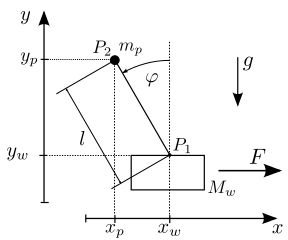
\includegraphics{inv_pendulum.png}

With the \emph{Lagrangian Formalism} the model has the following state space
representation where \(u_1 = F\) and
\(x = [x_1, x_2, x_3, x_4] = [x_w, \dot{x}_w, \varphi, \dot{\varphi}]\)
\begin{eqnarray*}
   \dot{x}_1 & = & x_2 \\
   \dot{x}_2 & = & \frac{m_p \sin(x_3)(-l x_4^2 + g \cos x_3)}{M_w l + m_p \sin^2(x_3)} + \frac{\cos(x_3)}{M_w l + m_p l \sin^2(x_3)} u_1 \\
   \dot{x}_3 & = & x_4 \\
   \dot{x}_4 & = & \frac{\sin(x_3)(-m_p l x_4^2 \cos(x_3) + g(M_w + m_p))}{M_w l + m_p \sin^2(x_3)} + \frac{\cos(x_3)}{M_w l + m_p l \sin^2(x_3)} u_1
\end{eqnarray*}
A possibly wanted trajectory is the translation of the cart along the
x-axis (i.e. by \(0.5m\)). In the beginning and end of the process
the cart and pendulum should remain at rest and the pendulum should be
aligned vertically upwards (\(\varphi = 0\)). As a further condition
\(u\) should start and end steadily in the rest position
(\(u(0) = u(T) = 0\)).
The operating time here is \(T = 1 [s]\).

\begin{Verbatim}[commandchars=\\\{\}]
\PYG{c}{\PYGZsh{} import trajectory class and necessary dependencies}
\PYG{k+kn}{from} \PYG{n+nn}{pytrajectory.trajectory} \PYG{k+kn}{import} \PYG{n}{Trajectory}
\PYG{k+kn}{from} \PYG{n+nn}{sympy} \PYG{k+kn}{import} \PYG{n}{sin}\PYG{p}{,} \PYG{n}{cos}
\PYG{k+kn}{import} \PYG{n+nn}{numpy} \PYG{k+kn}{as} \PYG{n+nn}{np}

\PYG{c}{\PYGZsh{} define the function that returns the vectorfield}
\PYG{k}{def} \PYG{n+nf}{f}\PYG{p}{(}\PYG{n}{x}\PYG{p}{,}\PYG{n}{u}\PYG{p}{)}\PYG{p}{:}
    \PYG{n}{x1}\PYG{p}{,} \PYG{n}{x2}\PYG{p}{,} \PYG{n}{x3}\PYG{p}{,} \PYG{n}{x4} \PYG{o}{=} \PYG{n}{x}       \PYG{c}{\PYGZsh{} system state variables}
    \PYG{n}{u1}\PYG{p}{,} \PYG{o}{=} \PYG{n}{u}                  \PYG{c}{\PYGZsh{} input variable}

    \PYG{n}{l} \PYG{o}{=} \PYG{l+m+mf}{0.5}     \PYG{c}{\PYGZsh{} length of the pendulum rod}
    \PYG{n}{g} \PYG{o}{=} \PYG{l+m+mf}{9.81}    \PYG{c}{\PYGZsh{} gravitational acceleration}
    \PYG{n}{M} \PYG{o}{=} \PYG{l+m+mf}{1.0}     \PYG{c}{\PYGZsh{} mass of the cart}
    \PYG{n}{m} \PYG{o}{=} \PYG{l+m+mf}{0.1}     \PYG{c}{\PYGZsh{} mass of the pendulum}

    \PYG{n}{s} \PYG{o}{=} \PYG{n}{sin}\PYG{p}{(}\PYG{n}{x3}\PYG{p}{)}
    \PYG{n}{c} \PYG{o}{=} \PYG{n}{cos}\PYG{p}{(}\PYG{n}{x3}\PYG{p}{)}

    \PYG{n}{ff} \PYG{o}{=} \PYG{n}{np}\PYG{o}{.}\PYG{n}{array}\PYG{p}{(}\PYG{p}{[}                     \PYG{n}{x2}\PYG{p}{,}
                   \PYG{n}{m}\PYG{o}{*}\PYG{n}{s}\PYG{o}{*}\PYG{p}{(}\PYG{o}{\PYGZhy{}}\PYG{n}{l}\PYG{o}{*}\PYG{n}{x4}\PYG{o}{*}\PYG{o}{*}\PYG{l+m+mi}{2}\PYG{o}{+}\PYG{n}{g}\PYG{o}{*}\PYG{n}{c}\PYG{p}{)}\PYG{o}{/}\PYG{p}{(}\PYG{n}{M}\PYG{o}{+}\PYG{n}{m}\PYG{o}{*}\PYG{n}{s}\PYG{o}{*}\PYG{o}{*}\PYG{l+m+mi}{2}\PYG{p}{)}\PYG{o}{+}\PYG{l+m+mi}{1}\PYG{o}{/}\PYG{p}{(}\PYG{n}{M}\PYG{o}{+}\PYG{n}{m}\PYG{o}{*}\PYG{n}{s}\PYG{o}{*}\PYG{o}{*}\PYG{l+m+mi}{2}\PYG{p}{)}\PYG{o}{*}\PYG{n}{u1}\PYG{p}{,}
                                        \PYG{n}{x4}\PYG{p}{,}
            \PYG{n}{s}\PYG{o}{*}\PYG{p}{(}\PYG{o}{\PYGZhy{}}\PYG{n}{m}\PYG{o}{*}\PYG{n}{l}\PYG{o}{*}\PYG{n}{x4}\PYG{o}{*}\PYG{o}{*}\PYG{l+m+mi}{2}\PYG{o}{*}\PYG{n}{c}\PYG{o}{+}\PYG{n}{g}\PYG{o}{*}\PYG{p}{(}\PYG{n}{M}\PYG{o}{+}\PYG{n}{m}\PYG{p}{)}\PYG{p}{)}\PYG{o}{/}\PYG{p}{(}\PYG{n}{M}\PYG{o}{*}\PYG{n}{l}\PYG{o}{+}\PYG{n}{m}\PYG{o}{*}\PYG{n}{l}\PYG{o}{*}\PYG{n}{s}\PYG{o}{*}\PYG{o}{*}\PYG{l+m+mi}{2}\PYG{p}{)}\PYG{o}{+}\PYG{n}{c}\PYG{o}{/}\PYG{p}{(}\PYG{n}{M}\PYG{o}{*}\PYG{n}{l}\PYG{o}{+}\PYG{n}{l}\PYG{o}{*}\PYG{n}{m}\PYG{o}{*}\PYG{n}{s}\PYG{o}{*}\PYG{o}{*}\PYG{l+m+mi}{2}\PYG{p}{)}\PYG{o}{*}\PYG{n}{u1}
                \PYG{p}{]}\PYG{p}{)}
    \PYG{k}{return} \PYG{n}{ff}

\PYG{c}{\PYGZsh{} boundary values at the start (a = 0.0 [s])}
\PYG{n}{xa} \PYG{o}{=} \PYG{p}{[}  \PYG{l+m+mf}{0.0}\PYG{p}{,}
        \PYG{l+m+mf}{0.0}\PYG{p}{,}
        \PYG{l+m+mf}{0.0}\PYG{p}{,}
        \PYG{l+m+mf}{0.0}\PYG{p}{]}

\PYG{c}{\PYGZsh{} boundary values at the end (b = 1.0 [s])}
\PYG{n}{xb} \PYG{o}{=} \PYG{p}{[}  \PYG{l+m+mf}{0.5}\PYG{p}{,}
        \PYG{l+m+mf}{0.0}\PYG{p}{,}
        \PYG{l+m+mf}{0.0}\PYG{p}{,}
        \PYG{l+m+mf}{0.0}\PYG{p}{]}

\PYG{c}{\PYGZsh{} create trajectory object}
\PYG{n}{T} \PYG{o}{=} \PYG{n}{Trajectory}\PYG{p}{(}\PYG{n}{f}\PYG{p}{,} \PYG{n}{a}\PYG{o}{=}\PYG{l+m+mf}{0.0}\PYG{p}{,} \PYG{n}{b}\PYG{o}{=}\PYG{l+m+mf}{1.0}\PYG{p}{,} \PYG{n}{xa}\PYG{o}{=}\PYG{n}{xa}\PYG{p}{,} \PYG{n}{xb}\PYG{o}{=}\PYG{n}{xb}\PYG{p}{)}

\PYG{c}{\PYGZsh{} run iteration}
\PYG{n}{T}\PYG{o}{.}\PYG{n}{startIteration}\PYG{p}{(}\PYG{p}{)}

\PYG{c}{\PYGZsh{} show results}
\PYG{n}{T}\PYG{o}{.}\PYG{n}{plot}\PYG{p}{(}\PYG{p}{)}
\end{Verbatim}


\chapter{PyTrajectory Modules Reference}
\label{pytrajectory:pytrajectory-modules-reference}\label{pytrajectory:module-pytrajectory}\label{pytrajectory::doc}\index{pytrajectory (module)}
PyTrajectory is a Python library for the determination of the feed forward control
to achieve a transition between desired states of a nonlinear control system.


\section{\texttt{trajectory} Module}
\label{pytrajectory:module-pytrajectory.trajectory}\label{pytrajectory:trajectory-module}\index{pytrajectory.trajectory (module)}\index{Trajectory (class in pytrajectory.trajectory)}

\begin{fulllineitems}
\phantomsection\label{pytrajectory:pytrajectory.trajectory.Trajectory}\pysiglinewithargsret{\strong{class }\code{pytrajectory.trajectory.}\bfcode{Trajectory}}{\emph{ff}, \emph{a=0.0}, \emph{b=1.0}, \emph{xa=None}, \emph{xb=None}, \emph{g=None}, \emph{sx=5}, \emph{su=5}, \emph{kx=2}, \emph{delta=2}, \emph{maxIt=7}, \emph{eps=0.01}, \emph{tol=1e-05}, \emph{algo='leven'}, \emph{use\_chains=True}}{}
Base class of the PyTrajectory project.
\begin{quote}\begin{description}
\item[{Parameters}] \leavevmode\begin{itemize}
\item {} 
\textbf{ff} (\emph{callable}) -- Vectorfield (rhs) of the control system

\item {} 
\textbf{a} (\emph{float}) -- Left border

\item {} 
\textbf{b} (\emph{float}) -- Right border

\item {} 
\textbf{xa} (\emph{list}) -- Boundary values at the left border

\item {} 
\textbf{xb} (\emph{list}) -- Boundary values at the right border

\item {} 
\textbf{g} (\emph{list}) -- Boundary values of the input variables

\item {} 
\textbf{sx} (\emph{int}) -- Initial number of spline parts for the system variables

\item {} 
\textbf{su} (\emph{int}) -- Initial number of spline parts for the input variables

\item {} 
\textbf{kx} (\emph{int}) -- Factor for raising the number of spline parts for the system variables

\item {} 
\textbf{delta} (\emph{int}) -- Constant for calculation of collocation points

\item {} 
\textbf{maxIt} (\emph{int}) -- Maximum number of iterations

\item {} 
\textbf{eps} (\emph{float}) -- Tolerance for the solution of the initial value problem

\item {} 
\textbf{tol} (\emph{float}) -- Tolerance for the solver of the equation system

\item {} 
\textbf{algo} (\emph{str}) -- Solver to use

\item {} 
\textbf{use\_chains} (\emph{bool}) -- Whether or not to use integrator chains

\end{itemize}

\end{description}\end{quote}
\index{DG() (pytrajectory.trajectory.Trajectory method)}

\begin{fulllineitems}
\phantomsection\label{pytrajectory:pytrajectory.trajectory.Trajectory.DG}\pysiglinewithargsret{\bfcode{DG}}{\emph{c}}{}
This is the callable function that returns the jacobian matrix of the collocation system.

\end{fulllineitems}

\index{G() (pytrajectory.trajectory.Trajectory method)}

\begin{fulllineitems}
\phantomsection\label{pytrajectory:pytrajectory.trajectory.Trajectory.G}\pysiglinewithargsret{\bfcode{G}}{\emph{c}}{}
This is the callable function that represents the collocation system.

\end{fulllineitems}

\index{analyseSystem() (pytrajectory.trajectory.Trajectory method)}

\begin{fulllineitems}
\phantomsection\label{pytrajectory:pytrajectory.trajectory.Trajectory.analyseSystem}\pysiglinewithargsret{\bfcode{analyseSystem}}{}{}
Analyses the systems structure and sets values for some of the method parameters.

\end{fulllineitems}

\index{buildEQS() (pytrajectory.trajectory.Trajectory method)}

\begin{fulllineitems}
\phantomsection\label{pytrajectory:pytrajectory.trajectory.Trajectory.buildEQS}\pysiglinewithargsret{\bfcode{buildEQS}}{}{}
Builds the collocation equation system.

\end{fulllineitems}

\index{checkAccuracy() (pytrajectory.trajectory.Trajectory method)}

\begin{fulllineitems}
\phantomsection\label{pytrajectory:pytrajectory.trajectory.Trajectory.checkAccuracy}\pysiglinewithargsret{\bfcode{checkAccuracy}}{}{}
Checks whether desired accuracy for the boundary values was reached.

\end{fulllineitems}

\index{dx() (pytrajectory.trajectory.Trajectory method)}

\begin{fulllineitems}
\phantomsection\label{pytrajectory:pytrajectory.trajectory.Trajectory.dx}\pysiglinewithargsret{\bfcode{dx}}{\emph{t}}{}
This function returns the left hand sites state at a given (time-) point \code{t}.

\end{fulllineitems}

\index{getGuess() (pytrajectory.trajectory.Trajectory method)}

\begin{fulllineitems}
\phantomsection\label{pytrajectory:pytrajectory.trajectory.Trajectory.getGuess}\pysiglinewithargsret{\bfcode{getGuess}}{}{}
This method is used to determine a starting value (guess) for the
solver of the collocation equation system --\textgreater{} docu p. 24

\end{fulllineitems}

\index{initSplines() (pytrajectory.trajectory.Trajectory method)}

\begin{fulllineitems}
\phantomsection\label{pytrajectory:pytrajectory.trajectory.Trajectory.initSplines}\pysiglinewithargsret{\bfcode{initSplines}}{}{}
This method is used to initialise the temporary splines

\end{fulllineitems}

\index{iterate() (pytrajectory.trajectory.Trajectory method)}

\begin{fulllineitems}
\phantomsection\label{pytrajectory:pytrajectory.trajectory.Trajectory.iterate}\pysiglinewithargsret{\bfcode{iterate}}{}{}
This method is used to run one iteration

\end{fulllineitems}

\index{plot() (pytrajectory.trajectory.Trajectory method)}

\begin{fulllineitems}
\phantomsection\label{pytrajectory:pytrajectory.trajectory.Trajectory.plot}\pysiglinewithargsret{\bfcode{plot}}{}{}
Just calls {\hyperref[pytrajectory:pytrajectory.trajectory.Trajectory.plot]{\code{plot()}}} function from \code{tools}

\end{fulllineitems}

\index{setCoeff() (pytrajectory.trajectory.Trajectory method)}

\begin{fulllineitems}
\phantomsection\label{pytrajectory:pytrajectory.trajectory.Trajectory.setCoeff}\pysiglinewithargsret{\bfcode{setCoeff}}{}{}
This method is used to create the actual splines by using the numerical
solutions to set up the coefficients of the polynomial spline parts of
every created spline.

\end{fulllineitems}

\index{simulate() (pytrajectory.trajectory.Trajectory method)}

\begin{fulllineitems}
\phantomsection\label{pytrajectory:pytrajectory.trajectory.Trajectory.simulate}\pysiglinewithargsret{\bfcode{simulate}}{}{}
This method is used to solve the initial value problem.

\end{fulllineitems}

\index{solve() (pytrajectory.trajectory.Trajectory method)}

\begin{fulllineitems}
\phantomsection\label{pytrajectory:pytrajectory.trajectory.Trajectory.solve}\pysiglinewithargsret{\bfcode{solve}}{}{}
This method is used to solve the collocation equation system.

\end{fulllineitems}

\index{startIteration() (pytrajectory.trajectory.Trajectory method)}

\begin{fulllineitems}
\phantomsection\label{pytrajectory:pytrajectory.trajectory.Trajectory.startIteration}\pysiglinewithargsret{\bfcode{startIteration}}{}{}
This is the main loop --\textgreater{} {[}5.1{]}

\end{fulllineitems}

\index{u() (pytrajectory.trajectory.Trajectory method)}

\begin{fulllineitems}
\phantomsection\label{pytrajectory:pytrajectory.trajectory.Trajectory.u}\pysiglinewithargsret{\bfcode{u}}{\emph{t}}{}
This function returns the inputs state at a given (time-) point \code{t}.

\end{fulllineitems}

\index{x() (pytrajectory.trajectory.Trajectory method)}

\begin{fulllineitems}
\phantomsection\label{pytrajectory:pytrajectory.trajectory.Trajectory.x}\pysiglinewithargsret{\bfcode{x}}{\emph{t}}{}
This function returns the system state at a given (time-) point \code{t}.

\end{fulllineitems}


\end{fulllineitems}



\section{\texttt{spline} Module}
\label{pytrajectory:spline-module}\label{pytrajectory:module-pytrajectory.spline}\index{pytrajectory.spline (module)}\index{CubicSpline (class in pytrajectory.spline)}

\begin{fulllineitems}
\phantomsection\label{pytrajectory:pytrajectory.spline.CubicSpline}\pysiglinewithargsret{\strong{class }\code{pytrajectory.spline.}\bfcode{CubicSpline}}{\emph{a=0.0}, \emph{b=1.0}, \emph{n=10}, \emph{tag='`}, \emph{bc=None}, \emph{bcd=None}, \emph{bcdd=None}, \emph{steady=True}}{}
This class provides an object that represents a cubic spline ...
\begin{quote}\begin{description}
\item[{Parameters}] \leavevmode\begin{itemize}
\item {} 
\textbf{a} (\emph{float}) -- Left border of spline interval.

\item {} 
\textbf{b} (\emph{float}) -- Right border of spline interval.

\item {} 
\textbf{n} (\emph{int}) -- Number of polynomial parts the spline will be devided into.

\item {} 
\textbf{tag} (\emph{str}) -- The `name' of the spline object.

\item {} 
\textbf{bc} (\emph{tuple}) -- Boundary values for the spline function itself.

\item {} 
\textbf{bcd} (\emph{tuple}) -- Boundary values for the splines 1st derivative

\item {} 
\textbf{bcdd} (\emph{tuple}) -- Boundary values for the splines 2nd derivative

\item {} 
\textbf{steady} (\emph{bool}) -- Whether or not to call {\hyperref[pytrajectory:pytrajectory.spline.CubicSpline.makesteady]{\code{makesteady()}}} when instanciated.

\end{itemize}

\end{description}\end{quote}
\index{dddf() (pytrajectory.spline.CubicSpline method)}

\begin{fulllineitems}
\phantomsection\label{pytrajectory:pytrajectory.spline.CubicSpline.dddf}\pysiglinewithargsret{\bfcode{dddf}}{\emph{x}}{}
This is just a wrapper for {\hyperref[pytrajectory:pytrajectory.spline.CubicSpline.evalf]{\code{evalf()}}} to evaluate the splines 3rd derivative.

\end{fulllineitems}

\index{ddf() (pytrajectory.spline.CubicSpline method)}

\begin{fulllineitems}
\phantomsection\label{pytrajectory:pytrajectory.spline.CubicSpline.ddf}\pysiglinewithargsret{\bfcode{ddf}}{\emph{x}}{}
This is just a wrapper for {\hyperref[pytrajectory:pytrajectory.spline.CubicSpline.evalf]{\code{evalf()}}} to evaluate the splines 2nd derivative.

\end{fulllineitems}

\index{df() (pytrajectory.spline.CubicSpline method)}

\begin{fulllineitems}
\phantomsection\label{pytrajectory:pytrajectory.spline.CubicSpline.df}\pysiglinewithargsret{\bfcode{df}}{\emph{x}}{}
This is just a wrapper for {\hyperref[pytrajectory:pytrajectory.spline.CubicSpline.evalf]{\code{evalf()}}} to evaluate the splines 1st derivative.

\end{fulllineitems}

\index{evalf() (pytrajectory.spline.CubicSpline method)}

\begin{fulllineitems}
\phantomsection\label{pytrajectory:pytrajectory.spline.CubicSpline.evalf}\pysiglinewithargsret{\bfcode{evalf}}{\emph{x}, \emph{d}}{}
bla bla bla
\begin{quote}\begin{description}
\item[{Parameters}] \leavevmode\begin{itemize}
\item {} 
\textbf{x} (\emph{float}) -- The point to evaluate the spline at

\item {} 
\textbf{d} (\emph{int}) -- The derivation order

\end{itemize}

\end{description}\end{quote}

\end{fulllineitems}

\index{f() (pytrajectory.spline.CubicSpline method)}

\begin{fulllineitems}
\phantomsection\label{pytrajectory:pytrajectory.spline.CubicSpline.f}\pysiglinewithargsret{\bfcode{f}}{\emph{x}}{}
This is just a wrapper for {\hyperref[pytrajectory:pytrajectory.spline.CubicSpline.evalf]{\code{evalf()}}} to evaluate the spline itself.

\end{fulllineitems}

\index{makesteady() (pytrajectory.spline.CubicSpline method)}

\begin{fulllineitems}
\phantomsection\label{pytrajectory:pytrajectory.spline.CubicSpline.makesteady}\pysiglinewithargsret{\bfcode{makesteady}}{}{}
This method sets up and solves equations that satisfy boundary conditions and
ensure steadiness and smoothness conditions of the spline in every joining point.

\end{fulllineitems}

\index{set\_coeffs() (pytrajectory.spline.CubicSpline method)}

\begin{fulllineitems}
\phantomsection\label{pytrajectory:pytrajectory.spline.CubicSpline.set_coeffs}\pysiglinewithargsret{\bfcode{set\_coeffs}}{\emph{c\_sol}}{}
This function is used to set up numerical values for the spline coefficients.
\begin{quote}\begin{description}
\item[{Parameters}] \leavevmode
\textbf{c\_sol} (\emph{dict}) -- Dictionary with coefficient and numerical value

\end{description}\end{quote}

\end{fulllineitems}

\index{tmp\_dddf() (pytrajectory.spline.CubicSpline method)}

\begin{fulllineitems}
\phantomsection\label{pytrajectory:pytrajectory.spline.CubicSpline.tmp_dddf}\pysiglinewithargsret{\bfcode{tmp\_dddf}}{\emph{x}}{}
This is just a wrapper for {\hyperref[pytrajectory:pytrajectory.spline.CubicSpline.tmp_evalf]{\code{tmp\_evalf()}}} with the splines 3rd derivative.

\end{fulllineitems}

\index{tmp\_ddf() (pytrajectory.spline.CubicSpline method)}

\begin{fulllineitems}
\phantomsection\label{pytrajectory:pytrajectory.spline.CubicSpline.tmp_ddf}\pysiglinewithargsret{\bfcode{tmp\_ddf}}{\emph{x}}{}
This is just a wrapper for {\hyperref[pytrajectory:pytrajectory.spline.CubicSpline.tmp_evalf]{\code{tmp\_evalf()}}} with the splines 2nd derivative.

\end{fulllineitems}

\index{tmp\_df() (pytrajectory.spline.CubicSpline method)}

\begin{fulllineitems}
\phantomsection\label{pytrajectory:pytrajectory.spline.CubicSpline.tmp_df}\pysiglinewithargsret{\bfcode{tmp\_df}}{\emph{x}}{}
This is just a wrapper for {\hyperref[pytrajectory:pytrajectory.spline.CubicSpline.tmp_evalf]{\code{tmp\_evalf()}}} with the splines 1st derivative.

\end{fulllineitems}

\index{tmp\_evalf() (pytrajectory.spline.CubicSpline method)}

\begin{fulllineitems}
\phantomsection\label{pytrajectory:pytrajectory.spline.CubicSpline.tmp_evalf}\pysiglinewithargsret{\bfcode{tmp\_evalf}}{\emph{x}, \emph{d}}{}
This function returns a matrix and vector to evaluate the spline or a derivative at x
by multiplying the matrix with numerical values of the independent variables
and adding the vector.
\begin{quote}\begin{description}
\item[{Parameters}] \leavevmode\begin{itemize}
\item {} 
\textbf{x} (\emph{real}) -- The point to evaluate the spline at

\item {} 
\textbf{d} (\emph{int}) -- The derivation order

\end{itemize}

\item[{Returns}] \leavevmode
Matrix and vector that represent how the splines coefficients depend on the free parameters.

\item[{Return type}] \leavevmode
tuple

\end{description}\end{quote}

\end{fulllineitems}

\index{tmp\_f() (pytrajectory.spline.CubicSpline method)}

\begin{fulllineitems}
\phantomsection\label{pytrajectory:pytrajectory.spline.CubicSpline.tmp_f}\pysiglinewithargsret{\bfcode{tmp\_f}}{\emph{x}}{}
This is just a wrapper for {\hyperref[pytrajectory:pytrajectory.spline.CubicSpline.tmp_evalf]{\code{tmp\_evalf()}}} with the spline itself.

\end{fulllineitems}


\end{fulllineitems}

\index{fdiff() (in module pytrajectory.spline)}

\begin{fulllineitems}
\phantomsection\label{pytrajectory:pytrajectory.spline.fdiff}\pysiglinewithargsret{\code{pytrajectory.spline.}\bfcode{fdiff}}{\emph{func}}{}
This function is used to get the derivative of of a callable splinefunction.
\begin{quote}\begin{description}
\end{description}\end{quote}

\end{fulllineitems}



\section{\texttt{solver} Module}
\label{pytrajectory:module-pytrajectory.solver}\label{pytrajectory:solver-module}\index{pytrajectory.solver (module)}\index{Solver (class in pytrajectory.solver)}

\begin{fulllineitems}
\phantomsection\label{pytrajectory:pytrajectory.solver.Solver}\pysiglinewithargsret{\strong{class }\code{pytrajectory.solver.}\bfcode{Solver}}{\emph{F}, \emph{DF}, \emph{x0}, \emph{tol=0.01}, \emph{maxx=10}, \emph{algo='leven'}}{}
This class provides solver for the collocation equation system.
\begin{quote}\begin{description}
\item[{Parameters}] \leavevmode\begin{itemize}
\item {} 
\textbf{F} (\emph{callable}) -- The callable function that represents the equation system

\item {} 
\textbf{DF} (\emph{callable}) -- The function for the jacobian matrix of the eqs

\item {} 
\textbf{x0} (\emph{numpy.ndarray}) -- The start value for the sover

\item {} 
\textbf{tol} (\emph{float}) -- The (absolute) tolerance of the solver

\item {} 
\textbf{maxx} (\emph{int}) -- The maximum number of iterations of the solver

\item {} 
\textbf{algo} (\emph{str}) -- The solver to use

\end{itemize}

\end{description}\end{quote}
\index{gauss() (pytrajectory.solver.Solver method)}

\begin{fulllineitems}
\phantomsection\label{pytrajectory:pytrajectory.solver.Solver.gauss}\pysiglinewithargsret{\bfcode{gauss}}{}{}
\end{fulllineitems}

\index{leven() (pytrajectory.solver.Solver method)}

\begin{fulllineitems}
\phantomsection\label{pytrajectory:pytrajectory.solver.Solver.leven}\pysiglinewithargsret{\bfcode{leven}}{}{}
This method is an implementation of the Levenberg-Marquardt-Method
to approximatively solve a system of non-linear equations by minimizing

\(\| F'(x_k)(x_{k+1} - x_k) + F(x_k) \|_2^2 + \mu^2 \|x_{k+1} - x_k \|\)

\end{fulllineitems}

\index{newton() (pytrajectory.solver.Solver method)}

\begin{fulllineitems}
\phantomsection\label{pytrajectory:pytrajectory.solver.Solver.newton}\pysiglinewithargsret{\bfcode{newton}}{}{}
\end{fulllineitems}

\index{solve() (pytrajectory.solver.Solver method)}

\begin{fulllineitems}
\phantomsection\label{pytrajectory:pytrajectory.solver.Solver.solve}\pysiglinewithargsret{\bfcode{solve}}{}{}
This is just a wrapper to call the chosen algorithm for solving the
equation system

\end{fulllineitems}


\end{fulllineitems}



\section{\texttt{simulation} Module}
\label{pytrajectory:module-pytrajectory.simulation}\label{pytrajectory:simulation-module}\index{pytrajectory.simulation (module)}\index{Simulation (class in pytrajectory.simulation)}

\begin{fulllineitems}
\phantomsection\label{pytrajectory:pytrajectory.simulation.Simulation}\pysiglinewithargsret{\strong{class }\code{pytrajectory.simulation.}\bfcode{Simulation}}{\emph{ff}, \emph{T}, \emph{start}, \emph{u}, \emph{dt=0.01}}{}
This class does something ...
\begin{quote}\begin{description}
\item[{Parameters}] \leavevmode\begin{itemize}
\item {} 
\textbf{ff} (\emph{callable}) -- Vectorfield of the control system

\item {} 
\textbf{T} (\emph{float}) -- Simulation time

\item {} 
\textbf{u} (\emph{callable}) -- Function of the input variables

\item {} 
\textbf{dt} (\emph{float}) -- Time step

\end{itemize}

\end{description}\end{quote}
\index{calcStep() (pytrajectory.simulation.Simulation method)}

\begin{fulllineitems}
\phantomsection\label{pytrajectory:pytrajectory.simulation.Simulation.calcStep}\pysiglinewithargsret{\bfcode{calcStep}}{}{}
\end{fulllineitems}

\index{rhs() (pytrajectory.simulation.Simulation method)}

\begin{fulllineitems}
\phantomsection\label{pytrajectory:pytrajectory.simulation.Simulation.rhs}\pysiglinewithargsret{\bfcode{rhs}}{\emph{t}, \emph{x}}{}
\end{fulllineitems}

\index{simulate() (pytrajectory.simulation.Simulation method)}

\begin{fulllineitems}
\phantomsection\label{pytrajectory:pytrajectory.simulation.Simulation.simulate}\pysiglinewithargsret{\bfcode{simulate}}{}{}
\end{fulllineitems}


\end{fulllineitems}



\section{\texttt{utilities} Module}
\label{pytrajectory:module-pytrajectory.utilities}\label{pytrajectory:utilities-module}\index{pytrajectory.utilities (module)}\index{BetweenDict (class in pytrajectory.utilities)}

\begin{fulllineitems}
\phantomsection\label{pytrajectory:pytrajectory.utilities.BetweenDict}\pysiglinewithargsret{\strong{class }\code{pytrajectory.utilities.}\bfcode{BetweenDict}}{\emph{d=\{\}}}{}
Bases: \code{dict}

\end{fulllineitems}

\index{Grid (class in pytrajectory.utilities)}

\begin{fulllineitems}
\phantomsection\label{pytrajectory:pytrajectory.utilities.Grid}\pysigline{\strong{class }\code{pytrajectory.utilities.}\bfcode{Grid}}
\end{fulllineitems}

\index{IntegChain (class in pytrajectory.utilities)}

\begin{fulllineitems}
\phantomsection\label{pytrajectory:pytrajectory.utilities.IntegChain}\pysiglinewithargsret{\strong{class }\code{pytrajectory.utilities.}\bfcode{IntegChain}}{\emph{lst}}{}
This class provides a representation of a integrator chain consisting of sympy symbols ...
\begin{quote}\begin{description}
\item[{Parameters}] \leavevmode
\textbf{lst} (\emph{lst}) -- Ordered list of elements for the integrator chain

\end{description}\end{quote}
\index{predecessor() (pytrajectory.utilities.IntegChain method)}

\begin{fulllineitems}
\phantomsection\label{pytrajectory:pytrajectory.utilities.IntegChain.predecessor}\pysiglinewithargsret{\bfcode{predecessor}}{\emph{elem}}{}
This method returns the predecessor of the given element of the
integrator chains, i.e. it returns \(\int [elem]\)
\begin{quote}\begin{description}
\item[{Parameters}] \leavevmode
\textbf{elem} (\emph{sympy.Symbol}) -- An element of the integrator chain

\end{description}\end{quote}

\end{fulllineitems}

\index{successor() (pytrajectory.utilities.IntegChain method)}

\begin{fulllineitems}
\phantomsection\label{pytrajectory:pytrajectory.utilities.IntegChain.successor}\pysiglinewithargsret{\bfcode{successor}}{\emph{elem}}{}
This method returns the successor of the given element of the
integrator chains, i.e. it returns \(\frac{d}{dt}[elem]\)
\begin{quote}\begin{description}
\item[{Parameters}] \leavevmode
\textbf{elem} (\emph{sympy.Symbol}) -- An element of the integrator chain

\end{description}\end{quote}

\end{fulllineitems}


\end{fulllineitems}

\index{Modell (class in pytrajectory.utilities)}

\begin{fulllineitems}
\phantomsection\label{pytrajectory:pytrajectory.utilities.Modell}\pysigline{\strong{class }\code{pytrajectory.utilities.}\bfcode{Modell}}~\index{draw() (pytrajectory.utilities.Modell method)}

\begin{fulllineitems}
\phantomsection\label{pytrajectory:pytrajectory.utilities.Modell.draw}\pysiglinewithargsret{\bfcode{draw}}{\emph{x}, \emph{phi}, \emph{frame}, \emph{image=0}}{}
\end{fulllineitems}


\end{fulllineitems}

\index{blockdiag() (in module pytrajectory.utilities)}

\begin{fulllineitems}
\phantomsection\label{pytrajectory:pytrajectory.utilities.blockdiag}\pysiglinewithargsret{\code{pytrajectory.utilities.}\bfcode{blockdiag}}{\emph{M}, \emph{bshape=None}, \emph{sparse=False}}{}
Takes block of shape \code{bshape}  from matrix \code{M} and creates
block diagonal matrix out of them.
\begin{quote}\begin{description}
\item[{Parameters}] \leavevmode\begin{itemize}
\item {} 
\textbf{M} (\emph{numpy.ndarray}) -- Matrix to take blocks from

\item {} 
\textbf{bshape} (\emph{tuple}) -- Shape of one block

\item {} 
\textbf{sparse} (\emph{bool}) -- Whether or not to return created matrix as sparse matrix

\end{itemize}

\end{description}\end{quote}
\paragraph{Examples}

\begin{Verbatim}[commandchars=\\\{\}]
\PYG{g+gp}{\PYGZgt{}\PYGZgt{}\PYGZgt{} }\PYG{n}{A} \PYG{o}{=} \PYG{n}{np}\PYG{o}{.}\PYG{n}{ones}\PYG{p}{(}\PYG{p}{(}\PYG{l+m+mi}{4}\PYG{p}{,} \PYG{l+m+mi}{2}\PYG{p}{)}\PYG{p}{)}
\PYG{g+gp}{\PYGZgt{}\PYGZgt{}\PYGZgt{} }\PYG{k}{print} \PYG{n}{A}
\PYG{g+go}{[[ 1.  1.]}
\PYG{g+go}{ [ 1.  1.]}
\PYG{g+go}{ [ 1.  1.]}
\PYG{g+go}{ [ 1.  1.]]}
\PYG{g+gp}{\PYGZgt{}\PYGZgt{}\PYGZgt{} }\PYG{n}{B} \PYG{o}{=} \PYG{n}{blockdiag}\PYG{p}{(}\PYG{n}{A}\PYG{p}{,} \PYG{p}{(}\PYG{l+m+mi}{2}\PYG{p}{,} \PYG{l+m+mi}{2}\PYG{p}{)}\PYG{p}{)}
\PYG{g+gp}{\PYGZgt{}\PYGZgt{}\PYGZgt{} }\PYG{k}{print} \PYG{n}{B}
\PYG{g+go}{[[ 1.  1.  0.  0.]}
\PYG{g+go}{ [ 1.  1.  0.  0.]}
\PYG{g+go}{ [ 0.  0.  1.  1.]}
\PYG{g+go}{ [ 0.  0.  1.  1.]]}
\end{Verbatim}

\end{fulllineitems}

\index{plot() (in module pytrajectory.utilities)}

\begin{fulllineitems}
\phantomsection\label{pytrajectory:pytrajectory.utilities.plot}\pysiglinewithargsret{\code{pytrajectory.utilities.}\bfcode{plot}}{\emph{sim}, \emph{H}, \emph{fname=None}}{}
This method provides graphics for each system variable, manipulated
variable and error function and plots the solution of the simulation.
\begin{quote}\begin{description}
\item[{Parameters}] \leavevmode\begin{itemize}
\item {} 
\textbf{sim} (\emph{tuple}) -- Contains collocation points, and simulation results of system and input variables

\item {} 
\textbf{H} (\emph{dict}) -- Dictionary of the callable error functions

\item {} 
\textbf{fname} (\emph{str (optional)}) -- If not None, plot will be saved as \textless{}fname\textgreater{}.png

\end{itemize}

\end{description}\end{quote}

\end{fulllineitems}

\index{struct (class in pytrajectory.utilities)}

\begin{fulllineitems}
\phantomsection\label{pytrajectory:pytrajectory.utilities.struct}\pysigline{\strong{class }\code{pytrajectory.utilities.}\bfcode{struct}}
\end{fulllineitems}



\section{\texttt{log} Module}
\label{pytrajectory:module-pytrajectory.log}\label{pytrajectory:log-module}\index{pytrajectory.log (module)}\index{IPS() (in module pytrajectory.log)}

\begin{fulllineitems}
\phantomsection\label{pytrajectory:pytrajectory.log.IPS}\pysiglinewithargsret{\code{pytrajectory.log.}\bfcode{IPS}}{\emph{loc=None}}{}
\end{fulllineitems}

\index{Logger (class in pytrajectory.log)}

\begin{fulllineitems}
\phantomsection\label{pytrajectory:pytrajectory.log.Logger}\pysiglinewithargsret{\strong{class }\code{pytrajectory.log.}\bfcode{Logger}}{\emph{fname}, \emph{mode}, \emph{suppress}}{}~\index{write() (pytrajectory.log.Logger method)}

\begin{fulllineitems}
\phantomsection\label{pytrajectory:pytrajectory.log.Logger.write}\pysiglinewithargsret{\bfcode{write}}{\emph{text}}{}
\end{fulllineitems}


\end{fulllineitems}

\index{Timer (class in pytrajectory.log)}

\begin{fulllineitems}
\phantomsection\label{pytrajectory:pytrajectory.log.Timer}\pysiglinewithargsret{\strong{class }\code{pytrajectory.log.}\bfcode{Timer}}{\emph{label='\textasciitilde{}'}, \emph{verbose=True}}{}
\end{fulllineitems}

\index{err() (in module pytrajectory.log)}

\begin{fulllineitems}
\phantomsection\label{pytrajectory:pytrajectory.log.err}\pysiglinewithargsret{\code{pytrajectory.log.}\bfcode{err}}{\emph{text}, \emph{lvl=0}}{}
\end{fulllineitems}

\index{info() (in module pytrajectory.log)}

\begin{fulllineitems}
\phantomsection\label{pytrajectory:pytrajectory.log.info}\pysiglinewithargsret{\code{pytrajectory.log.}\bfcode{info}}{\emph{text}, \emph{lvl=0}}{}
\end{fulllineitems}

\index{logtime() (in module pytrajectory.log)}

\begin{fulllineitems}
\phantomsection\label{pytrajectory:pytrajectory.log.logtime}\pysiglinewithargsret{\code{pytrajectory.log.}\bfcode{logtime}}{\emph{text}, \emph{lvl=0}}{}
\end{fulllineitems}

\index{msg() (in module pytrajectory.log)}

\begin{fulllineitems}
\phantomsection\label{pytrajectory:pytrajectory.log.msg}\pysiglinewithargsret{\code{pytrajectory.log.}\bfcode{msg}}{\emph{label}, \emph{text}, \emph{lvl=0}}{}
\end{fulllineitems}

\index{set\_file() (in module pytrajectory.log)}

\begin{fulllineitems}
\phantomsection\label{pytrajectory:pytrajectory.log.set_file}\pysiglinewithargsret{\code{pytrajectory.log.}\bfcode{set\_file}}{\emph{fname='/usr/bin/sphinx-build2\_140407-200320.log'}, \emph{suppress=False}}{}
\end{fulllineitems}

\index{warn() (in module pytrajectory.log)}

\begin{fulllineitems}
\phantomsection\label{pytrajectory:pytrajectory.log.warn}\pysiglinewithargsret{\code{pytrajectory.log.}\bfcode{warn}}{\emph{text}, \emph{lvl=0}}{}
\end{fulllineitems}



\chapter{Indices and tables}
\label{index:indices-and-tables}\begin{itemize}
\item {} 
\emph{genindex}

\item {} 
\emph{modindex}

\item {} 
\emph{search}

\end{itemize}


\renewcommand{\indexname}{Python Module Index}
\begin{theindex}
\def\bigletter#1{{\Large\sffamily#1}\nopagebreak\vspace{1mm}}
\bigletter{p}
\item {\texttt{pytrajectory}}, \pageref{pytrajectory:module-pytrajectory}
\item {\texttt{pytrajectory.log}}, \pageref{pytrajectory:module-pytrajectory.log}
\item {\texttt{pytrajectory.simulation}}, \pageref{pytrajectory:module-pytrajectory.simulation}
\item {\texttt{pytrajectory.solver}}, \pageref{pytrajectory:module-pytrajectory.solver}
\item {\texttt{pytrajectory.spline}}, \pageref{pytrajectory:module-pytrajectory.spline}
\item {\texttt{pytrajectory.trajectory}}, \pageref{pytrajectory:module-pytrajectory.trajectory}
\item {\texttt{pytrajectory.utilities}}, \pageref{pytrajectory:module-pytrajectory.utilities}
\end{theindex}

\renewcommand{\indexname}{Index}
\printindex
\end{document}
